\section{Methodology}

\subsection{Profiling}
Before attempting to accelerate a model like DALES, the most time-consuming parts of the code should be identified. This process is called profiling, for which various tools exist. NVIDIA NSight Systems is such a tool, and is particularly well-suited for GPU applications \citep{nvidiaNVIDIANsightSystems}. NSys automatically tracks CPU-GPU interactions, including data transfer and GPU utilization, but does not track CPU utilization. To track CPU activity, a custom timer module based on the NVIDIA Tools Extension (NVTX) library is used. With NVTX, CPU code can be tracked by NSys as well. The necessary code for NVTX has been added to DALES already. NSys comes with a GUI to visually inspect the profile (\autoref{fig:nsys}), which will be used to track the performance of DALES as its components are offloaded to the GPU.

\begin{figure}[H]
    \centering
    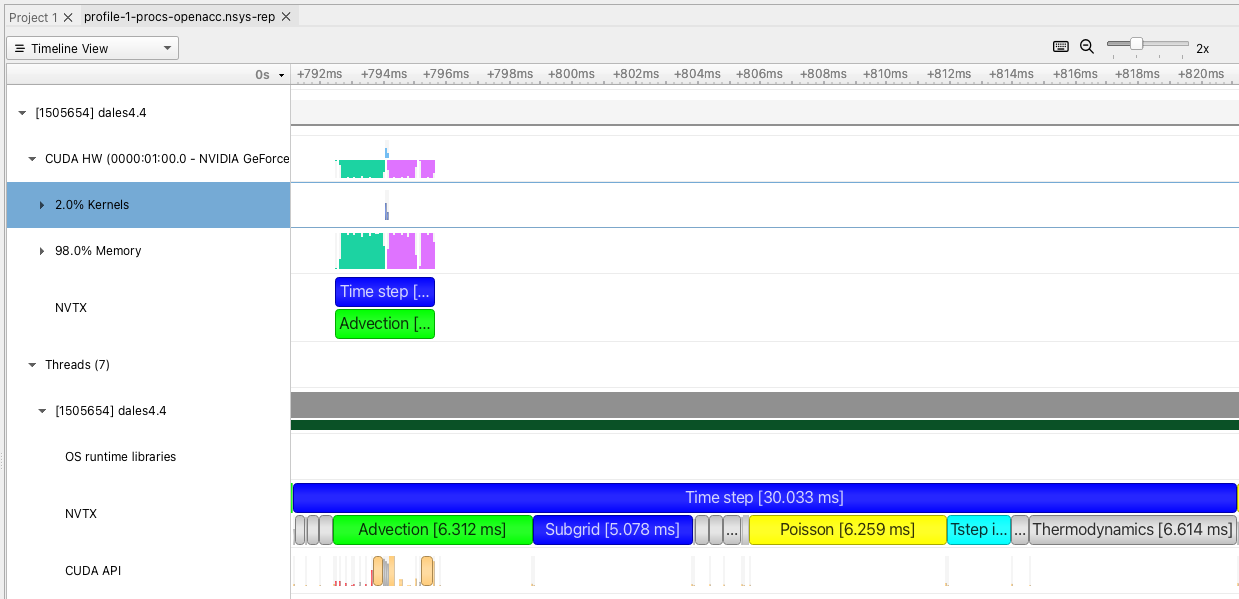
\includegraphics[width=0.9\textwidth]{doc/images/profiles/nsys.png}
    \caption{A screenshot of the NSys GUI. The main subroutine calls in DALES' time steps have been annotated with NVTX markers and show up at the bottom of the image, with their execution time between brackets. To demonstrate the GPU tracking capabilities of NSys, one advection kernel has been offloaded to the GPU (\texttt{advecu\_2nd}), which shows up under ``CUDA HW''. It can be seen that NSys automatically separates kernel execution time from time spent on memory operations, allowing for easy identification of performance bottlenecks.}
    \label{fig:nsys}
\end{figure}

\subsection{OpenACC}
According to the literature, OpenACC is a straightforward programming model to implement into an existing code base, while still offering good performance, especially when data transfers are properly optimized. This makes it a good choice for accelerating DALES. In \autoref{fig:nsys} a profile of DALES can be found. It can be seen that during a single time step, most time is spent on advection, sub-grid, Poisson, and thermodynamics modules. These modules involve parallelizable loops, making them well-suited for OpenACC.

The first step in getting DALES running on GPUs is to place OpenACC directives over all parallelizable loops. An example of a loop with an OpenACC directive can be found in \autoref{listing:accloop}. Once a loop or a group of loops has been offloaded, the data transfers can be optimized. As mentioned previously, memory transfers between CPU and GPU can contribute significantly to the wall-clock time of an application. Hence, it is important to minimize the amount of data transfers and optimize data locality (i.e., the location of data). With OpenACC, the programmer does not have to be explicit about data transfers, as the compiler can determine when to move data by itself. However, to ensure optimal data locality, it is good practice to explicitly copy data to and from the GPU. In OpenACC, this is also done via compiler directives. This approach will also be applied to DALES. Ideally, all fields will be copied to the GPU before the time loop begins, and data will only be copied back to the CPU for writing output files, with no additional data transfer in between. This may not be possible to realize for DALES, as some algorithms may not be parallelizable, meaning that these are better run on the CPU. In this case, intermediate data transfers are required.

\begin{listing}[H]
\begin{minted}{fortran}
!$acc parallel loop collapse(3) default(present)
do k = 1, kmax
    do j = 1, jmax
        do i = 1, imax
            c(i,j,k) = a(i,j,k) + b(i,j,k)
        end do
    end do
end do
\end{minted}
\caption{Example of a Fortran loop decorated with an OpenACC directive. The directive \texttt{!\$acc parallel loop} tells the compiler that the following loop can be executed in parallel. The \texttt{collapse(3)} clause collapses the three nested loops into one big loop, exposing more parallelism, and the \texttt{default(present)} clause tells the compiler that the arrays \texttt{a}, \texttt{b} and \texttt{c} already exist on the GPU and no further data transfer is needed.}
\label{listing:accloop}
\end{listing}

\subsection{Solving the Poisson equation}

In DALES, a solution for the pressure $\pi$ is obtained by solving the following Poisson equation:

\begin{equation}
    \frac{\partial^2 \pi}{\partial x_i^2} = \frac{\partial }{\partial x_i} \left( - \frac{\partial \overline{u}_i \overline{u}_j}{\partial x_j} + \frac{g}{\theta_0}\overline{\theta}_v\delta_{i3} + \mathcal{F}_i - \frac{\partial \tau_{ij}}{\partial x_j} \right) \label{eq:pressure}
\end{equation}

DALES provides two methods to solve this equation: using Fast Fourier Transforms (FFTs), or using iterative solvers. Among these, the FFT-based solver is the fastest. DALES has the ability to use the highly optimized Fastest Fourier Transform in the West (FFTW) library \citep{FFTW97}. FFTW is not capable of running on GPUs, however. NVIDIA provides an FFT library in their HPC SDK called cuFFT, which does run on GPUs and can be used instead of FFTW. cuFFT has a similar interface as FFTW, making the conversion straightforward.

\subsection{Multiple GPUs}
Currently, DALES is parallelized with MPI by decomposing the domain into slabs or pencils. OpenACC introduces further parallelization by distributing loop iterations among GPU threads. This means that MPI and OpenACC can be combined to run DALES on more than one GPU, for example by decomposing the domain into a number of slabs or pencils that equals the number of available GPUs, with each MPI process bound to its own GPU. An important thing to note is that the communication overhead increases with this approach, as halo transfers now also include copying data from GPU to CPU in addition to communication between CPUs. To mitigate this performance penalty to some degree, an MPI implementation that is aware of GPU memory can be used, which combines and optimizes the data transfer and MPI call.

The FFT-based Poisson equation solver relies heavily on communication between processes (and therefore, GPUs). This is because it requires transposing the data in between FFT calculations, which in turn requires a redistribution of the data. Currently, the transpose operations are implemented manually in DALES, using MPI \texttt{Alltoall} operations. When FFTW is replaced by cuFFT, these transpose operations must also be adopted for the GPU. Alternatively, the multi-process version of cuFFT, cuFFTMp, can be used. This library enables multi-process, multi-GPU FFTs, without the need to transpose the data and perform \texttt{MPI\_Alltoall} manually. In fact, inter-GPU communication is optimized using another communication library called NVSHMEM \citep{nvidiadeveloperNVSHMEM}, which offers superior performance compared to regular MPI communications. cuFFTMp can bind to an existing MPI communicator, and handle data transposition internally. Yet another option is to use the cuDecomp library as described by \citet{romeroDistributedmemorySimulationsTurbulent2022}. cuDecomp does not offer any FFT functionality but functions as an abstraction layer for the domain decomposition and communications. Given a certain number of MPI processes, cuDecomp automatically determines the optimal domain decomposition. For example, given 32 processes, a 3D domain can be decomposed into 1$\times$32, 2$\times$16, or 4$\times$8 chunks, each potentially yielding different performance. Additionally, cuDecomp supports multiple communication backends (MPI, NVSHMEM, NCCL), from which it selects the best performing during run time. This can improve performance significantly, especially when GPUs are distributed over multiple nodes. Because of its promising performance benefits on current-generation supercomputers, implementing cuDecomp is an objective of this project.

\newpage

\subsection{Verification and performance testing}
Modifying source code carries the risk of introducing bugs. While OpenACC requires minimal rewriting of source code, some modifications may be necessary for optimization purposes. Therefore, the updated source code needs to be validated against the original unmodified code to ensure that the program logic stays intact. Because of the chaotic nature of turbulence, one cannot simply perform an element-wise comparison of two arrays after a number of time steps. Instead, for some simulation case, multiple runs will be done, each with identical settings but different random seeding. From these runs, ensemble statistics can be calculated, like the mean and standard deviation of a quantity. The correctness of the modified code can be verified by comparing the value of some quantity against its mean from the ensemble; if the value is located within two standard deviations (95\% confidence interval) from the ensemble mean, one can say that the modified code remains correct with a reasonable level of certainty. Multiple cases will be validated, as different cases can stress the components of DALES differently. 

There are multiple metrics available to define the performance of a GPU program. One obvious metric is the speedup in the wall-clock time of using one CPU versus using one GPU for multiple grid sizes. When using more than one GPU, the scaling of the wall-clock time with the number of GPUs used is a good indication of the parallel efficiency. The scaling is measured by calculating the speedup that is gained from using more GPUs for a fixed problem size. As for the verification, this will also be done for multiple cases.